%% ------------------------------------------------------------------------- %%
\chapter{Tecnologias}
\label{cap:tecnologias}
\section{Ruby on Rails}
\subsection{Ruby}
    \par A criação da linguagem Ruby data de 1995 no Japão por Yukihiro ``Matz'' Matsumoto sob forte influência de outras linguagens como Perl, SmallTalk, Eiffel, Ada e Lisp.  Inicialmente o objetivo era equilibrar programação funcional, imperativa e orientação a objetos \citep{rubydocs}.
\begin{itemize}
\item{Flexibilidade:}
    \par A Linguagem Ruby cresceu devido a sua grande flexibilidade. Sendo possível alterar, remover ou acrescentar partes da linguagem à vontade.
    \par Como no seguinte exemplo: um usuário prefere utilizar a palavra \emph{plus} ao invés do operador matemático `` + '', ele poderia então adicionar esse método à classe nativa do Ruby Numeric pois os operadores matemáticos são considerados açúcares sintáticos nesta linguagem.
\\Exemplo:
\begin{lstlisting}[frame=single]
class Numeric
          def plus(x)
                self.+(x)
          end
    end

    y = 5.plus 6
    # y agora é igual a 11
\end{lstlisting}
\item{Closures:}
\par Nesta linguagem, closures são chamadas de blocos e são funções que podem ser tratadas como uma variável. Isso quer dizer que podem ser passadas como argumentos de métodos, serem atribuídas a outras variáveis, etc.
\par As closures armazenam os valores das variáveis que estavam no escopo quando a função foi definida e são capazes de acessar tais variáveis mesmo que sejam executadas em um escopo diferente\footnote{Fonte: Site Point \url{https://www.sitepoint.com/closures-ruby/} Acesso em: 29 ago. 2016.}.
\\
Exemplo:
\begin{lstlisting}[frame=single]
search_engines =
  %w[Google Yahoo MSN].map do |engine|
    "http://www." + engine.downcase + ".com"
  end
\end{lstlisting}
\item{Módulos:}
\par Módulos são formas de agrupar métodos, classes e constantes prevenindo conflitos de nomes e permitindo a fácil implementação de Mixins.
\par Diferente de outras linguagens orientadas a objetos Ruby suporta apenas herança simples porém isso é contornado através dos Mixins que permitem à uma classe receber mais de um módulo diferente, herdando assim todos seus métodos e definições.
\\Exemplo:
\begin{lstlisting}[frame=single]
class MyArray
          include Enumerable
    end
\end{lstlisting}

\end{itemize}
\subsection{Rails}

\par Ruby on Rails é um arcabouço escrito em linguagem Ruby, implementado seguindo o padrão MVC\footnote{Modelo-Visão-Controlador: Na qual o Modelo é a camada que contém os dados e lógica da aplicação, a Visão é a camada de entrada e saída de dados e o Controlador faz a conexão entre ambas camadas, fonte: \url{https://pt.wikipedia.org/wiki/MVC} Acesso em: 29 ago. 2016.} totalmente \emph{server-side}, sendo considerado portanto um arcabouço \emph{back-end}.
\par Este arcabouço oferece também uma estrutura para banco de dados \emph{web service} e \emph{web pages}, além de encorajar padrões de engenharia de software já consagrados tais como\footnote{Fonte: Ruby on Rails \url{https://en.wikipedia.org/wiki/Ruby_on_Rails} Acesso em: 29 ago. 2016.}
\begin{itemize}
\item {\emph{Convention over Configuration} (CoC):}
    \par Convenções de configuração visando padronizar o código. Ao adicionar convenções é retirada do desenvolvedor a decisão de como usar o arcabouço porém isso não diminui sua flexibilidade. Por exemplo ao criar-se um objeto chamado ``User'' então sua tabela por convenção se chamará ``users'' e o correspondente \emph{controller} será UsersController ( no plural) pois esse é padrão definido pelo arcabouço.
    \par Vale ressaltar que é possível alterar essas convenções para adaptar-se às necessidades do desenvolvedor.

\item {\emph{Don't Repeat yourself} (DRY):}
    \par É definido como ``Todo pedaço de informação deve ter uma única, não ambígua, representação autorizada com o Sistema'' \footnote{Fonte: Wikipedia \url{https://en.wikipedia.org/wiki/Don\%27t_repeat_yourself} Acesso em: 29 ago. 2016.}.
    \par Isso significa que uma modificação em uma parte do sistema não deve modificar outra parte não relacionada assim como elementos que são logicamente relacionados quando modificados ocorrem de forma previsível e uniforme.

\item { \emph{Active Record Pattern}:}
    \par O padrão Active Record sugere uma interface específica para acessar objetos em um banco de dados relacional contendo funções tais como INSERT, UPDATE, DELETE, etc. Uma tabela ou \emph{view} será associada a uma classe e então uma instância de objeto estará associada a uma única entrada na respectiva tabela.
    \par Em Ruby on Rails a biblioteca ActiveRecord implementa o padrão ORM além de acrescentar herança e associações, resolvendo dois problemas substanciais do padrão. ActiveRecord é o \emph{model} padrão do componente MVC, porém é possível trocá-lo por outra implementação do arcabouço Rails caso o desenvolvedor prefira.
\end{itemize}
    \par Em um sentido mais amplo Rails é mais que uma biblioteca de software ou API: é um projeto central de uma vasta comunidade que produz \emph{plugins} para facilitar e construir projetos complexos.
	\par As bibliotecas criadas pela comunidade para serem usadas em conjunto com o Rails são distribuídas em código aberto e chamadas de Ruby Gems ou apenas Gems\footnote{Fonte: Wikipedia \url{https://en.wikipedia.org/wiki/RubyGems} Acesso em: 29 ago. 2016.}.

\section{Heroku}
\par Heroku é uma PaaS implementada utilizando \emph{cloud computing} criada em 2007 utilizada como um modelo de \emph{Deployment} para Aplicações Web\footnote{Fonte: Heroku \url{https://en.wikipedia.org/wiki/Heroku} Acesso em: 29 ago. 2016.}.
\par  A aplicação é enviada para o Heroku por meio de uma conexão direta via GitHub, Dropbox ou alguma outra API e então rede do Heroku executa os aplicativos em containers virtuais.
\par Enviado o código-fonte ele então é convertido em uma aplicação interpretando as dependências de outras bibliotecas seguindo o padrão de cada linguagem.  No caso do USP Eventos que foi feito utilizando Ruby as dependências ficam armazenadas no próprio Gemfile da aplicação.
\par Feito o \emph{upload} da aplicação um container com uma virtualização de Unix é disponibilizado, chamado de Dyno da aplicação. Tal container é pré-carregado com algumas configurações da aplicação tais como um nome gerado automaticamente, variáveis de ambiente e \emph{add-ons} se existirem.
\par O Heroku então inicializa o Dyno com a aplicação, carrega-a e então realiza o \emph{deploy} da mesma. Dessa forma através do DNS \emph{Server} oferecido pelo próprio Heroku a aplicação fica acessível por meio de um domínio na forma <nome da aplicação>.herokuapp.com sendo possível redirecionar seu domínio particular para refletir o DNS disponibilizado.
\section{Travis CI}
\par Travis CI é um serviço de integração contínua usado para testar projetos hospedados no Github. Toda vez que um commit é feito para o repositório selecionado no Gitbhub o Travis executa as diretrizes especificadas no arquivo travis.yml que contém os comandos necessários para rodar os testes automatizados da aplicação, como é o caso do USP Eventos (figura \ref{fig:travis}).
\begin{figure}[htb]
\centering
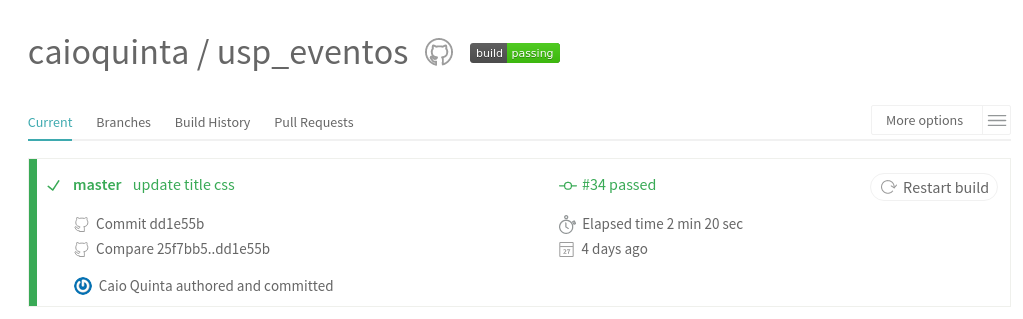
\includegraphics[width=15cm]{figuras/travis}
\caption{\label{fig:travis} O repositório USP Eventos no Travis CI.}
\end{figure}

\section{Trello}
\par Trello (www.trello.com) é um gerenciador de projetos online desenvolvido pela Fog Creek Software lançado em 2011. Possui uma interface amigável na qual é possível criar tarefas e colunas conforme as preferências do usuário sendo bastante utilizado em conjunto com uma abordagem \emph{kanban} para gerenciamento.

\section{Github}
\par Github é um serviço que disponibiliza repositórios git baseado na \emph{web} lançado em 2008. O serviço de controle de versão é implementado pelo git enquanto o Github implementa outras funcionalidades próprias como gerenciamento de tarefas, wikis próprias e \emph{bug tracking}.
\par É possível integrar o seu repositório no Github com outros serviços. No caso do USP Eventos o repositório no Github foi integrado com o Travis CI e também com o próprio Heroku (figura \ref{fig:heroku_automatic_deploy}).
\par Dessa forma caso um \emph{commit} para a \emph{branch} ``Produção'' fosse aprovado pelo Travis CI então o Heroku automaticamente colocava-o em produção.
\begin{figure}[htb]
\centering
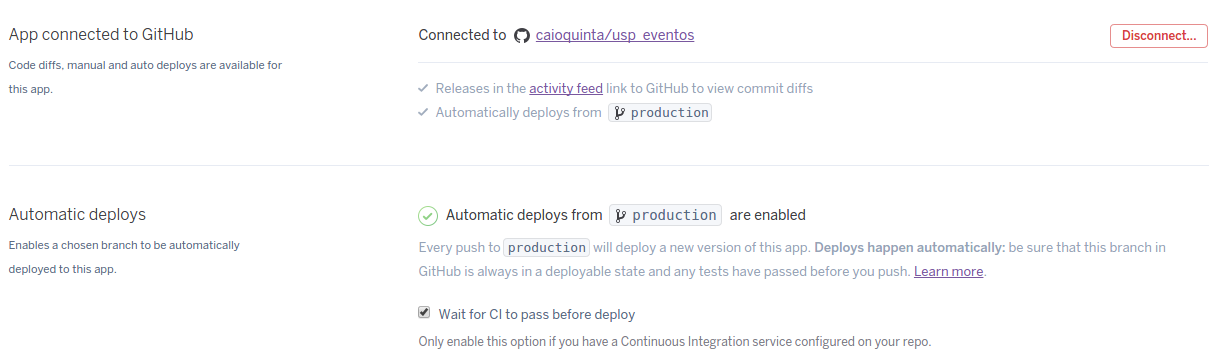
\includegraphics[width=15cm]{figuras/heroku_automatic_deploy}
\caption{\label{fig:heroku_automatic_deploy} Tela de Administração do Heroku para integração com o Github e \emph{deploy} automático.}
\end{figure}
\section{Google Analytics e Google Tag Manager}
\par O Google Analytics é uma plataforma de análise de dados oferecida pelo Google que permite por meio dos relatórios gerados pela plataforma obter uma série de informações quanto ao tipo de usuário que visualiza a página, o fluxo do site e a origem do acesso.
\par Com o uso de \emph{tags} é possível criar eventos que são personalizados e disparados de acordo com a navegação do usuário dentro do site. Tais \emph{tags} podem ser implementadas diretamente com um pequeno código em javascript para integração com o Google Analytics ou utilizando o Google Tag Manager.
\par O Google Tag Manager é uma plataforma intermediária que provê acesso e configuração de tags personalizadas para obtenção de dados pelo Google Analytics sem que seja necessário modificar diretamente o código-fonte do sistema. A opção de utilizar o Google Tag Manager no projeto deu-se principalmente pela facilidade de criar-se novas tags e alterações além de garantir uma maior organização das informações.
\par Dentro do projeto foi utilizado as informações obtidas pelo Google Analytics para validação de aprendizado entre as iterações.

\section{Painel de opiniões Populares - POP}
\par Com o intuito de definir o interesse do público alvo por meio de uma enquete colaborativa, foi utilizado o POP como sistema de votação devido a possibilidade dos usuários poderem adicionar itens à enquete principal.
\par Desenvolvido por estudantes do próprio IME dentro da disciplina de Laboratório de Programação Extrema à pedido da INDX o POP é uma plataforma de pesquisa de opinião pública que possui o objetivo realizar enquetes junto à comunidades para auxiliar na tomada de decisões e encaminhamento de opiniões para as autoridades responsáveis.
\par Foi permitida a utilização da plataforma implementada em uma instância separada com o nome de POP-TCC realizando apenas uma pequena modificação no sistema POP original.
\par No POP-TCC os usuários só poderiam votar de maneira positiva nas opções ao contrário do sistema original que permitia votos negativos e até ocultamento dos itens que obtivessem um grande número de negativações pelos usuários.

\section{HeatMap}
\par O serviço fornecido pela plataforma Heatmap.me consiste em prover uma API que é capaz de capturar os cliques em uma determinada página e mostrá-los na forma de uma mapa de calor.
\par Um mapa de calor é uma representação gráfica dos cliques em uma página na qual conforme uma determinada região for recebendo mais cliques sua cor é alterada proporcionalmente(figura \ref{fig:heatmap_explanation}).
\begin{figure}[htb]
\centering
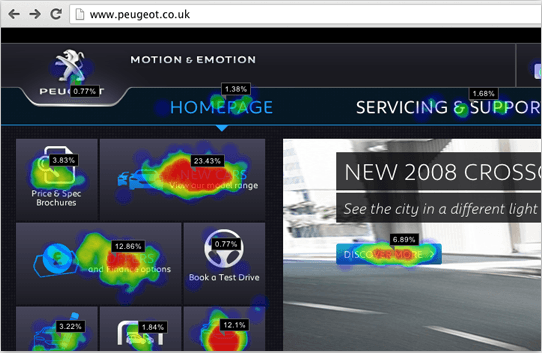
\includegraphics[width=15cm]{figuras/heatmap_explanation}
\caption{\label{fig:heatmap_explanation} Um exemplo de uma página utilizando o HeatMap.}
\end{figure}
\par As cores inicialmente começam em um tom verde quando clicadas poucas vezes sendo gradativamente alteradas para cores mais ``quentes'' tais como laranja ou vermelho conforme cliques na mesma região são feitos.

\section{Typeform}
\par A empresa Typeform oferece um serviço de formulários online para execução de pesquisas simples ou complexas.
\par A ferramenta é adequada para entrevistas de satisfação e opinião do cliente, oferecendo uma interface gráfica bastante amigável além de templates configuráveis para o tipo de pesquisa que o usuário deseja realizar.
\par Após a execução da pesquisa é possível exportar os resultados em planilhas ou integrar com o seu banco de dados caso desejar.
